\chapter{USB}
El \emph{Universal Serial Bus}(USB\footnote{V\'ease - http://www.usb.org}) es
un bus serial ent\'andar que hace de interfaz entre un dispositivo y una
computadora.
Dicha estandarizaci\'on es llevada acabo por el \emph{F\'orum de
Implementadores de USB} (USB Implementers Forum, USB-IF\footnote{V\'ease -
http://www.usb.org/about}). 
Actualmente el est\'andar se encuentra en su versi\'on 3.0\footnote{V\'ease -
http://www.usb.org/developers/docs/}, aunque la mayor\'ia de las
implementaciones comerciales solo soportan el ent\'andar \emph{2.0}.

\section{Historia}
%No me gusta como titulo 'historia' habria que pensar otra cosa

\section{Decripci\'on}
% Aca iria el funcionamiento del USB, difierenciado por \subsection{}
% Por ahora me estoy basando en la spec 2.0 oficial.
La especificaci\'on USB provee una serie de atributos con los cuales se pueden
implementar dispositivos seg\'un el precio/rendimiento deseado.

\subsection{Caracter\'isticas}
Del amplio rango de caracter\'isticas definidas en el ent\'andar, es posible
agruparlas en ocho categor\'ias:
% Reescribir lo de arriba y agregar mas

\begin{itemize}
 \item Facilidad de uso para el usuario final
 \item Amplio rango de aplicaciones
 \item Ancho de banda is\'ocrono
 \item Flexibilidad
 \item Robustez
 \item Sinergia con la industria de la PC
 \item Implementaci\'on de bajo costo
 \item De arquitectura actualizable
\end{itemize}

La combinaci\'on de estas caracter\'isticas hacen a la versatilidad del
ent\'andar, ya que permiten implementar todo tipo de dispositivos seg\'un la
carga, versatilidad, eficiencia, precio, velocidad y dem\'as atributos que
puedan inferir en un diese\~no.

\subsection{Arquitectura}

USB es un \emph{bus} cableado que soporta conexiones entre un \emph{host} y
gran rango de perif\'ericos. Dicho \emph{bus} permite la conexi\'on,
configuraci\'on, uso y desconexi\'on de un dispositivo mientras el \emph{host}
y dem\'as perif\'ericos est\'an en funcionamiento. \\

Un sistema USB se  define segun tres grandes \'areas:

\begin{itemize}
 \item Interconexi\'on USB
 \item Dispositivo USB
 \item \emph{Host} USB
\end{itemize}

\subsection{Interconexi\'on USB}

La interconexi\'on USB define la manera en la que los dispositivos USB se
conectan entre si y con el \emph{host}. 

\subsubsection{Topolog\'ia del bus}

USB usa una topolog\'ia de estrella por niveles. Un \emph{hub}\footnote{La
palabra \emph{hub} se traduce al castellano como \emph{centro}, pero su
traducci\'on no sera usada en este documento por cuestiones pr\'acticas.}
est\'a ubicado al centro de cada estrella. Las conexiones cableadas se dan
entre el \emph{host} y un \emph{hub} o funci\'on, entre \emph{hub} y
\emph{hub}, o entre un \emph{hub} y una funci\'on. \\

Debido a cuestiones de tiempo, el n\'umero maximo de niveles permitido es
siete, incluida la ra\'iz. La figura \ref{fig:usb_topology} muestra un esquema
de la topolog\'ia.

\begin{figure}
\centering
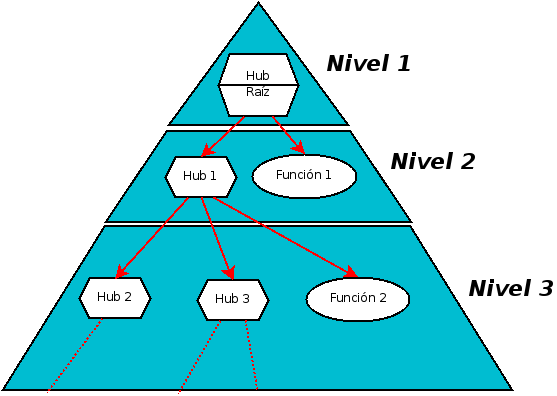
\includegraphics[scale=0.5]{./img/usb_topology.png}
\caption{Topolog\'ia del bus USB.}
\label{fig:usb_topology}
\end{figure}

\subsection{\emph{Host} USB}

La especificaci\'on admite un solo \emph{Host} para un todo sistema USB. La
interf\'az USB del \emph{host}, se la denomina \emph{Host
Controller}\footnote{Al igual que con \emph{host}, esta palabra se mantedr\'a
en ingles.}. La implementaci\'on de un \emph{Host Controller} puede ser una
combinaci\'on de hardware, firmware o software. El \emph{hub} ra\'iz esta
integrado en el sistema \emph{host}, proveyendo puntos de acceso.

\subsection{Dispositivo USB}

Los dispositivos USB pueden ser dispositivos funcionales o bien \emph{hubs}.
En ambos casos deben ser capaces de entender el protocolo USB y responder a
peticiones estandares USB ademas de cumplir su funci\'on intr\'inseca. 

% Explicar --- UHCI, OHCI, EHCI
\begin{Huge} TERMINAR!!! \end{Huge}


\section{USB en linux}

Linux comenz\'o a soportar el protocolo USB desde la versi\'on 2.2.7
(\emph{principio de 1999}), con codigo aportado por el mismo \emph{Linus
Torvalds\footnote{Codigo fuente
en: ftp://ftp.kernel.org/pub/linux/kernel/testing/old/usb/}
\footnote{V\'ease:
http://marc.info/?l=linux-usb\&m=92282561930486\&w=2}
}.\\

Con el paso del tiempo el soporte de linux para el protoco USB ha aumentado
considerablemente, y actualmente existen drivers para una enorme cantidad de
dispositivos.\\

Linux interpone varias capas de abstracci\'on entre el usuario y el hardware
USB, en la figura \ref{fig:usb_linux_layers} se puede apreciar una
representacion de dichas capas.

\begin{figure}
\centering
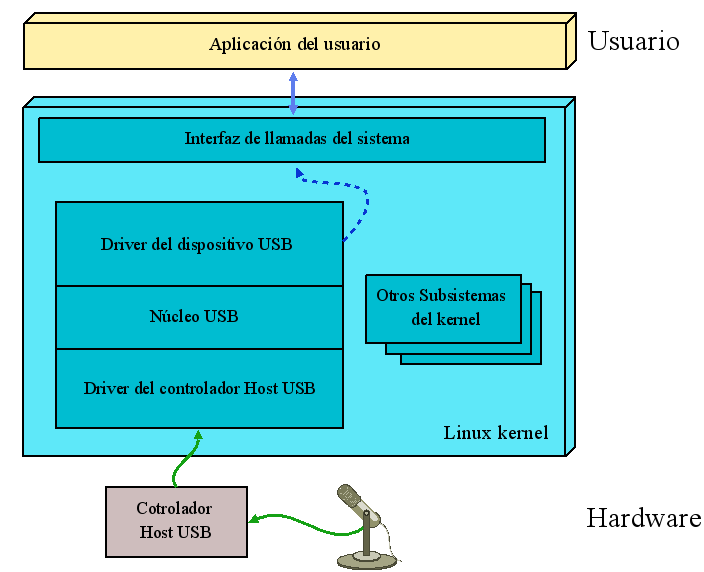
\includegraphics[scale=0.5]{./img/usb_linux_layers.png}
\caption{Soporte USB de linux.}
\label{fig:usb_linux_layers}
\end{figure}


En los cap\'itulos siguientes se describir\'a como es
manejado el protocolo a nivel del kernel y una \emph{API} libre de mas alto
nivel.


\subsection{Manejo USB de bajo nivel}

El kernel linux posee documentaci\'on embebida, la cual puede ser generada en
formato \emph{postscipt} \footnote{V\'ease -
http://es.wikipedia.org/wiki/PostScript}, pdf, o html. Para lograr esto basta
con bajar el codigo del kernel y compilar la documentaci\'on de la siguiente
manera:


\begin{scriptsize}
	\begin{verbatim}
	$ wget http://www.kernel.org/pub/linux/kernel/v2.6/linux-x.y.z.tar.bz2
	$ tar -xjf linux-x.y.z.tar.bz2
	$ cd  linux-x.y.z/
	$ make pdfdocs
	\end{verbatim}
\end{scriptsize}

En la documentaci\'on generada se encuentra una secci\'on espec\'ifica sobre
USB.\\

Basicamente linux posee en su nivel m\'as bajo drivers para el controlador
host (ya sean UHCI, OHCI o EHCI), el cual se comunica con el
\emph{usbcore}\footnote{Tambi\'en llamado API, pero aqui nos referiremos como
\emph{usbcore} o \emph{core} por cuestiones pr\'acticas.} quien interactua
directamente con los drivers espec\'ificos de cada dispositivo (Ver figura
\ref{fig:usb_linux_layers}).


